\section{Обзор предметной области}

В данной секции представлена базовая теория запросов к графам с КС ограничениями,
рассмотрены существующие алгоритмы выполнения данных запросов, с акцентом на перспективное направление алгоритмов, которые полагаются на операции разреженной линейной алгебры. Также в данной секции рассмотрен алгоритм поиска путей на основе тензорного произведении, а также представлены существующие инструменты для работы с примитивами разреженной линейной алгебры на GPGPU, и обоснована необходимость разработки нового подобного инструмента.

\subsection{Терминология}

% В этой секции изложены основные определения и факты из теории графов и формальных языков, необходимые для понимания предметной области. 
    
\textit{Ориентированный граф с метками на ребрах} $\mathcal{G} = \langle V, E, L \rangle$ это тройка объектов, где $V$ конечное непустое множество вершин графа, $E \subseteq V \times L \times V$ конечное множество ребер графа, $L$ конечное множество меток графа. Здесь и далее будем считать, что вершины графа индексируются целыми числами, т.е. $V = \{0~...~|V| - 1\}$.

Граф $\mathcal{G} = \langle V, E, L \rangle$ можно представить в виде матрицы смежности $M$ размером $|V| \times |V|$, где $M[i,j] = \{l~|~(i,l,j) \in E\}$. Используя булеву матричную декомпозицию, можно представить матрицу смежности в виде набора матриц $\mathcal{M} = \{ M^l ~|~ l \in L, M^l[i,j] = 1 \iff l \in M[i,j]\}$.

Путь $\pi$ в графе $\mathcal{G} = \langle V, E, L \rangle$ это последовательность ребер $e_0,e_1,e_{n-1}$, где $e_i = (v_i, l_i, u_i) \in E$ и для любых $e_i, e_{i+1}: u_i = v_{i+1}$. Путь между вершинами $v$ и $u$ будем обозначать как $v \pi u$. Слово, которое формирует путь $\pi = (v_0, l_0, v_1), ... ,(v_{n-1}, l_{n-1}, v_n)$ будем обозначать как $\omega (\pi) = l_0 ... l_{n-1}$, что является конкатенацией меток вдоль этого пути $\pi$.

\textit{Контекстно-свободная (КС) грамматика} $G = \langle \Sigma, N, P, S \rangle$ это четверка объектов, где $\Sigma$ конечное множестве терминалов или терминальный алфавит, $N$ конечное множество нетерминалов, $P$ конечное множество правил вывода вида $A \rightarrow \gamma, \gamma \in (N \cup \Sigma)^*$, $S \in N$ стартовый нетерминал. Вывод слова $w$ в грамматике из нетерминала $S$ применением одного или нескольких правил вывода обозначается как $S \rightarrow^*_G w$.

Язык $\mathcal{L}$ над конечным алфавитом символов $\Sigma$ --- множество слов, составленных из символов этого алфавита, т.е. $\mathcal{L} \subseteq \{w~|~w \in \Sigma ^*\}$. Язык, задаваемый грамматикой $G$, обозначим как $\mathcal{L}(G) = \{w~|~S \rightarrow^*_G w\}$.

% Keep this thing commented
% \begin{figure}[h]
%     \centering
%     \begin{subfigure}[b]{0.50\textwidth}
%         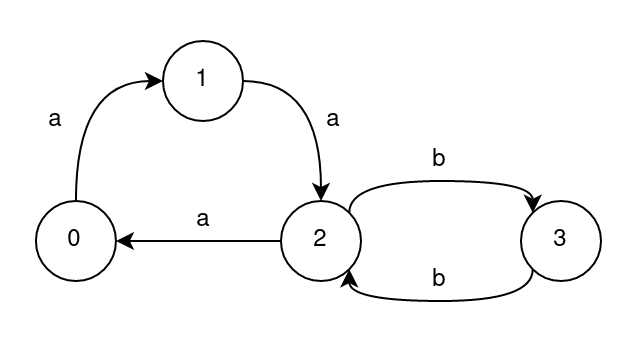
\includegraphics[width=\textwidth]{images/example_graph.png}
%         \caption{Ориентированный граф с меткам}
%     \end{subfigure}
%     \hfill
%     \begin{subfigure}[b]{0.20\textwidth}
%         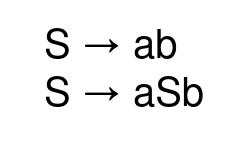
\includegraphics[width=\textwidth]{images/exmample_grammar.png}
%         \caption{Грамматика}
%     \end{subfigure}
%     \caption{Пример графа и грамматики}
% \end{figure}

\subsection{Поиск путей с ограничениями}

При вычислении запроса на поиск путей в графе $\mathcal{G} = \langle V, E, L \rangle$ в качестве ограничения выступает некоторый язык $\mathcal{L}$, которому должны удовлетворять результирующие пути.

Поиск путей в графе с семантикой \textbf{достижимости} --- это поиск всех таких пар вершин $(v,u)$, что между ними существует путь $v \pi u$ такой, что $\omega (\pi) \in \mathcal{L}$. Результат запроса обозначается как $R = \{ (v,u)~|~\exists v \pi u : \omega (\pi) \in \mathcal{L} \}$.

Поиск путей в графе с семантикой \textbf{всех путей} --- это поиск всех таких путей $v \pi u$,   что $\omega (\pi) \in \mathcal{L}$. Результат запроса обозначается как $\Pi = \{ v \pi u~|~v \pi u : \omega (\pi) \in \mathcal{L} \}$.
Необходимо отметить, что множество $\Pi$ может быть бесконечным, поэтому в качестве результата запроса предполагается не всё множество в явном виде, а некоторый \textit{итератор}, который позволит последовательно извлекать все пути.

Семантика \textbf{одного пути} является ослабленной формулировкой семантики всех путей, так как для получения результата достаточно найти всего один путь вида $v \pi u : \omega (\pi) \in \mathcal{L}$ для каждой пары $(v, u) \in R$.

Поскольку язык $\mathcal{L}$ может быть бесконечным, при составлении запросов используют не множество $\mathcal{L}$ в явном виде, а некоторое правило формирования слов этого языка. В качестве таких правил и выступают регулярные выражения или КС грамматики. При именовании запросов отталкиваются от типа правил, поэтому запросы именуются как регулярные или КС соответственно.

\subsection{Существующие решения}

Впервые проблема выполнения запросов с контекстно-свободными ограничениями была сформулирована в 1990 году в работе Михалиса Яннакакиса~\cite{inproceedings:yannakakis_cfpq_problem}. С того времени были представлены многие работы, в которых так или иначе предлагалось решение данной проблемы. 

Однако недавно  Йохем Куиджперс и др.~\cite{article:kuijpers_cfpq_exp_compare} на основе сравнения нескольких алгоритмов~\cite{article:hellings_cfpq,inproceedings:matrix_cfpq,inbook:santos_cfpq_lr_analysis} для выполнения запросов с контекстно-свободными ограничениями заключили, что существующие алгоритмы неприменимы для практики из-за проблем с производительностью.
Стоит отметить, что алгоритмы, используемые в статье, были реализованы на языке программирования \textit{Java} и исполнялись в среде \textit{JVM} в однопоточном режиме, что могло существенно повлиять на производительность представленных алгоритмов и, соответственно, выводы авторов.

Это подтверждают результаты работы Арсения Терехова и др.~\cite{inproceedings:cfqp_matrix_with_single_source}, в которой с использованием программных и аппаратных средств Nvidia Cuda был реализован алгоритм Рустама Азимова~\cite{inproceedings:matrix_cfpq}. В данном алгоритме задача поиска путей с КС ограничениями была сведена к операциям линейной алгебры, что позволило использовать высокопроизводительные библиотеки для выполнения данных операций на GPGPU. 
Данное исследование показывает, что эффективная реализация алгоритма на GPU может сделать его применимым для анализа реальных данных.


Алгоритм Рустама Азимова~\cite{inproceedings:cfqp_matrix_with_single_source} способен выполнять запросы только в семантике одного пути. Поскольку в качестве формализма для представления грамматики КС запроса используется \textit{ослабленная нормальная форма Хомского (ОНФХ)}~\cite{book:automata_theory}, увеличение числа правил в исходной грамматике запроса может приводить к существенному разрастанию ОНФХ, что негативно влияет на время работы алгоритма.

\subsection{Поиск путей с КС ограничениями через тензорное произведение}

Представленный в работе Егора Орачева и др.~\cite{inbook:kronecker_cfpq_adbis} алгоритм для выполнения КС запросов использует операции линейной булевой алгебры: произведение Кронекера (частный случай тензорного произведения), матричное умножение и сложение. Данный алгоритм позволяет выполнять запросы в семантике достижимости и всех путей, а также он подходит для реализации на многоядерных системах, что делает его потенциально применимым для анализа реальных данных. Кроме этого, данный алгоритм использует в качестве формализма для представления запроса \textit{рекурсивный автомат} (РА)~\cite{article:recursive_state_machines}, что потенциально может решить проблему разрастания исходной грамматики запроса. 

Идея алгоритма состоит в \textit{пересечении} РА и графа с использованием некоторой модификации классического алгоритма пересечения рекурсивных автоматов~\cite{book:automata_theory}. Пересечение выполняется с использованием произведения Кронекера, а множество рекурсивных вызовов учитывается с помощью транзитивного замыкания, что также выражается с использованием матричных операций умножения и поэлементного сложения. Данный процесс итеративный, и он выполняется до тех пор, пока в результирующий граф добавляются новые ребра.

% Далее предлагается рассмотреть описание данного алгоритма и используемую им технику сведения вычислений к операциям линейной алгебры.

% \subsubsection*{Рекурсивный автомат}

% Для представления входной грамматики КС запроса алгоритм~\cite{inbook:kronecker_cfpq_adbis} использует \textit{рекурсивный автомат}. Данный формализм является своего рода обобщением \textit{недетерминированного конечного автомата} на случай КС языков. Для понимания того, как он устроен, обратимся к теории формальных языков.

% \textit{Недетерминированный конечный автомат} (НКА) $F = \langle \Sigma, Q, Q_s, Q_f, \delta \rangle$ это пятерка объектов, где:

% \begin{itemize}
%     \item $\Sigma$ конечное множество входных символов или алфавит
%     \item $Q$ конечное множество состояний
%     \item $Q_s \subseteq Q$ множество стартовых состояний
%     \item $Q_f \subseteq Q$ множество конечных состояний
%     \item $\delta : \Sigma \times Q \rightarrow 2^Q$ функция переходов автомата
% \end{itemize}

% Язык, допускаемый автоматом $F$ будем обозначать как $L(F)$. Любое регулярное выражение может быть преобразовано в соответствующий НКА~\cite{book:automata_theory}. 

% \textit{Рекурсивный автомат} (РА) $R = \langle M, m, \{C_i\}_{i \in M} \rangle$ это тройка объектов, где: 

% \begin{itemize}
%     \item $M$ конечное множество меток компонентных НКА, называемых далее \textit{модули}
%     \item $m$ метка стартового модуля
%     \item $\{C_i\}$ множество модулей, где модуль $C_i = \langle \Sigma \cup M, Q_i, S_i, F_i, \delta _i \rangle$ состоит из:
%     {
%     \begin{itemize}
%         \item $\Sigma \cup M$ множество символов модуля, $\Sigma \cap M = \emptyset$
%         \item $Q_i$ конечное множество состояний модуля, $Q_i \cap Q_j = \emptyset, \forall i \neq j$
%         \item $S_i \subseteq Q_i$ множество стартовых состояний модуля
%         \item $F_i \subseteq Q_i$ множество конечных состояний модуля 
%         \item $\delta_i : (\Sigma \cup M) \times Q_i \rightarrow 2^{Q_i}$ функция переходов
%     \end{itemize}
%     }
% \end{itemize}

% Рекурсивный автомат ведет себя как набор НКА или модулей~\cite{article:recursive_state_machines}. Эти модули очень сходны с НКА при обработке входных последовательностей символов, однако они способны обрабатывать дополнительные \textit{рекурсивные вызовы} за счет неявного \textit{стека вызовов}, который присутствует во время работы РА. С точки зрения прикладного программиста это похоже на рекурсивные вызовы одних функций из других с той разницей, что вместо функций здесь выступают модули РА.

% Рекурсивные автоматы по своей вычислительной мощности эквивалентны магазинным автоматам~\cite{article:recursive_state_machines}. А поскольку подобный магазинный автомат способен распознавать КС грамматику~\cite{book:automata_theory}, рекурсивные автоматы эквивалентны КС грамматикам. Это позволяет корректно использовать РА для представления входной КС грамматики запроса.

% \subsubsection*{Пересечение рекурсивного автомата и графа}

% Классический алгоритм~\cite{book:automata_theory} \textit{пересечения} двух НКА $F^1$ и $F^2$ позволяет построить новый НКА $F$ с таким свойством, что он допускает пересечение исходных регулярных языков, т.е. $L(F) = L(F^1) \cap L(F^2)$. Формально, для $F^1 = \langle \Sigma, Q^1, Q^1_S, Q^1_F, \delta^1 \rangle$ и $F^2 = \langle \Sigma, Q^2, Q^2_S, Q^2_F, \delta^2 \rangle$ строится новый НКА $F = \langle \Sigma, Q, Q_S, Q_F, \delta \rangle$, где:

% \begin{itemize}
%     \item $Q = Q^1 \times Q^2$
%     \item $Q_S = Q^1_S \times Q^2_S$
%     \item $Q_F = Q^1_F \times Q^2_F$
%     \item $\delta: \Sigma \times Q \rightarrow Q$ и $\delta(s, \langle q_1, q_2 \rangle) = \langle q'_1, q'_2 \rangle$, если $\delta^1 (s, q_1)=q'_1$ и $\delta^2 (s, q_2)=q'_2$ 
% \end{itemize}

% Интерпретируя ориентированный граф с метками как некоторый конечный автомат, в котором все вершины графа являются одновременно начальными и конечными состояниями автомата, а ребра графа --- переходами между состояниями автомата, возможно пересечь этот граф и некоторый НКА, используя алгоритм пересечения, описанный выше. Однако, если представить граф и функцию переходов КА, тоже интерпретируемую как граф, в виде матриц смежности, можно использовать \textit{произведение Кронекера} для построения функции переходов автомата пересечения.

% \textit{Произведение Кронекера} для двух матриц $A$ и $B$ размера $m_1 \times n_1$ и $m_2 \times n_2$ с поэлементной операцией умножения $\cdot$ дает матрицу $M = A \otimes B$ размером $m_1 * m_2 \times n_1 * n_2$, где $M[u * m_2 + v, p * n_2 + q] = A[u, p] \cdot B[v, q]$. 

% Поскольку РА состоит из набора модулей, которые по своей структуре не сильно отличаются от классических НКА, это дает идею для применения похожего алгоритма пересечения РА и графа, с той  разницей, что процесс пересечения будет итеративным и будет включать в себя транзитивное замыкание, чтобы учесть \textit{рекурсивные вызовы}, присутствующие в РА. 

% \subsubsection*{Описание алгоритма}

В листинге~\ref{tensor:cfpq} представлен псевдокод алгоритма. Необходимо отметить, что алгоритм использует булеву матричную декомпозицию в строках \textbf{3 -- 4} для представления матрицы переходов РА и матрицы смежности графа, а также использует матричное умножение, сложение и произведение Кронекера в строках \textbf{14 -- 16}.

Данный алгоритм является относительно простым в реализации, так как всю сложность выполнения он перекладывает на операции линейной алгебры, которые должны быть реализованы в сторонних высокопроизводительных библиотеках.

\begin{algorithm}[h]
\floatname{algorithm}{Listing}
\begin{algorithmic}[1]
\footnotesize
\caption{Поиск путей через произведение Кронекера}
\label{tensor:cfpq}
\Function{KroneckerProductBasedCFPQ}{G, $\mathcal{G}$}
    % Input data preparation
    \State{$R \gets$ Рекурсивный автомат для грамматики $G$}
    \State{$\mathcal{M}_1 \gets$ Матрица переходов $R$ в булевой форме}
    \State{$\mathcal{M}_2 \gets$ Матрица смежности $\mathcal{G}$ в булевой форме}
    \State{$C_3 \gets$ Пустая матрица}
    % Eps-transition handling for graph
    \For{$s \in \{0,...,dim(\mathcal{M}_1)-1\}$}
        \For{$S \in \textit{getNonterminals}(R,s,s)$}
            \For{$i \in \{0,...,dim(\mathcal{M}_2)-1\}$}
                % Or just $M_2^n[i,i] \gets M_2^n[i,i] \vee \{1\}$ ??? 
                \State{$M_2^S[i,i] \gets \{1\}$}
            \EndFor
        \EndFor
    \EndFor
    \While{Матрица смежности $\mathcal{M}_2$ изменяется}
        % Kronecker product (i.e. partial intersection)
        \State{$\mathcal{M}_3 \gets \mathcal{M}_1 \otimes \mathcal{M}_2$}
        \Comment{Вычисление произведения Кронекера}
        % Collapse to single Boolean matrix
        \State{$M'_3 \gets \bigvee_{M_3^a \in \mathcal{M}_3} M_3^a $}
        \Comment{Слияние матриц в одну булеву матрицу достижимости}
        % Closure over Boolean matrix only
        \State{$C_3 \gets \textit{transitiveClosure}(M'_3)$}
        \Comment{Транзитивное замыкание для учета рекурсивных вызовов}
        \State{$n \times n \gets$ dim($M_3)$}
        % Add non-terminals (possibly new)
        \For{$(i,j)~|~C[i,j] \neq 0$}
            \State{$s, f \gets \textit{getStates}(C_3,i,j)$}
            \State{$x, y \gets \textit{getCoordinates}(C_3,i,j)$}
            \For{$S \in \textit{getNonterminals}(R,s,f)$}
                \State{$M_2^S[x,y] \gets \{1\}$}
            \EndFor
        \EndFor
    \EndWhile
\State \Return $\mathcal{M}_2,C_3$
\EndFunction
\end{algorithmic}
\end{algorithm}

% Keep this thing commented
% \begin{algorithm}[]
% \floatname{algorithm}{Listing}
% \begin{algorithmic}[1]
% \footnotesize
% \caption{Вспомогательные функции для алгоритма поиска путей}
% \label{tensor:cfpq:help}
% \Function{GetStates}{$C, i, j$}
%     \State{$r \gets dim(\mathcal{M}_1)$}
%     \Comment{$\mathcal{M}_1$ матрица переходов в булевой форме для $R$}
%     \State \Return{$\left\lfloor{i / r}\right\rfloor, \left\lfloor{j / r}\right\rfloor$}
% \EndFunction
% \Function{GetCoordinates}{$C, i, j$}
%     \State{$n \gets dim(\mathcal{M}_2)$}
%     \Comment{$\mathcal{M}_2$ матрица смежности в булевой форме для $\mathcal{G}$}
%     \State \Return{$i \bmod n, j \bmod n$}
% \EndFunction
% \end{algorithmic}
% \end{algorithm}

% todo: paths extraction algorithm
% \subsection{Извлечение всех путей}

\subsection{Вычисления на GPGPU}

\textit{GPGPU} (от англ. General-purpose computing on graphics processing units) --- техника использования графического процессора видеокарты компьютера для осуществления неспециализированных вычислений, 
которые обычно проводит центральный процессор. 
Данная техника позволяет получить значительной прирост производительности в SIMD (англ. single instruction, multiple data) вычислениях, 
когда необходимо обрабатывать большие массивы однотипных данных с фиксированным набором команд.

Исторически видеокарты в первую очередь использовались как графические ускорители для создания высококачественной трехмерной графики в режиме реального времени. Позже стало ясно, что мощность графического процессора можно использовать не только для графических вычислений. Так появились программируемые вычислительные блоки (англ. compute shaders), которые позволяют выполнять на видеокарте неграфические вычисления.

На данный момент существует несколько промышленных стандартов для создания программ, использующих графический процессор, одними из которых являются Vulkan~\cite{net:spec_vulkan}, OpenGL~\cite{net:spec_opengl}, DirectX~\cite{net:spec_direct3d} как API для графических и неспециализированных вычислительных задач, а также OpenCL~\cite{net:spec_opencl}, Nvidia Cuda~\cite{net:cuda_toolkit_docs} как API для неспециализированных вычислений. 

В качестве технологии для GPGPU в этой работе используется Nvidia Cuda. В то время как OpenCL создавался как кросс-платформенный стандарт для программирования вычислений, Cuda API специфичен только для видеокарт производства компании Nvidia. Однако он имеет более широкий набор инструментов как для написания, так и для отладки программ, а также собственный компилятор NVCC, который позволяет осуществлять кросс-компиляцию кода на языке Cuda C/C++, и прозрачно использовать его вместе с кодом на языке C/C++. Кроме этого, в данной работе используется результаты исследования Арсения Терехова и др.~\cite{inproceedings:cfqp_matrix_with_single_source}, в котором также использовалось Cuda API.

\subsection{Примитивы разреженной линейной алгебры для GPGPU}

Для эффективной реализации алгоритмов~\cite{inbook:kronecker_cfpq_adbis, inproceedings:matrix_cfpq} требуются высокопроизводительные библиотеки операций линейной алгебры. 
Реальные графовые данные насчитывают порядка $10^5$ -- $10^9$ вершин и являются сильно разреженными, т.е. количество ребер в графе сравнимо с количеством вершин, поэтому плотные матрицы не подходят для представления такого типа данных. 

% В качестве такой библиотеки для выполнения матричных операций на центральном процессоре авторы исследований~\cite{inbook:kronecker_cfpq_adbis, inproceedings:cfqp_matrix_with_single_source} использовали \textit{SuiteSparse}~\cite{article:suite_sparse_for_graph_problems}. Это эталонная реализация стандарта \textit{GraphBLAS}~\cite{paper:graphblas_foundations}, который был разработан как некоторый инструмент для реализации алгоритмов обработки графов на языке линейной алгебры.  

% Экспериментальное исследование~\cite{inproceedings:cfpq_matrix_evaluation} по реализации алгоритма Рустама Азимова~\cite{inproceedings:matrix_cfpq} на GPGPU с использованием операций над плотными булевыми матрицами показало, что вычисление на графическом процессоре дает значительный прирост производительности при обработке синтетических данных и данных среднего размера. Однако реальные графовые данные насчитывают порядка $10^5$ -- $10^9$ вершин и являются сильно разреженными, т.е. количество ребер в графе сравнимо с количеством вершин, поэтому плотные матрицы не подходят для представления такого типа данных. 

Библиотеки \textit{cuSPARSE}~\cite{net:cusparse_docs} и \textit{CUSP}~\cite{net:cusplibrary} для платформы Nvidia Cuda и \textit{clSPARSE}~\cite{10.1145/2909437.2909442} для платформы OpenCL предоставляют функциональность для работы с разреженными данными, однако они фокусируются на обработке численных данных и специализируются только на стандартных типах, таких как \textit{float}, \textit{double}, \textit{int} и \textit{long}. Для реализации алгоритмов~\cite{inbook:kronecker_cfpq_adbis, inproceedings:matrix_cfpq} требуются операции над разреженными булевыми матрицами, поэтому требуется специализация вышеуказанных библиотек для работы с булевыми примитивами. С одной стороны, библиотека cuSPARSE имеет закрытый исходный код, что делает невозможным ее модификацию, с другой стороны, библиотеки CUSP и clSPARSE имеет открытый исходный код и свободную лицензию, однако используемые ими алгоритмы умножения разреженных матриц \textit{достаточно} требовательны к ресурсам памяти~\cite{inproceedings:cfqp_matrix_with_single_source}, что делает их неприменимым для обработки данных большого размера.

Также необходимо отметить такие библиотеки как \textit{GraphBLAST}~\cite{yang2019graphblast} и \textit{bhSPARSE}~\cite{10.1016/j.jpdc.2015.06.010}. GraphBLAST является попыткой реализовать стандарт GraphBLAS~\cite{paper:graphblas_foundations} --- промышленный API для анализа графов в терминах линейной алгебры. Данный стандарт позволят использовать произвольные полукольца для вычислений, включая булево полукольцо. bhSPARSE предоставляет реализацию примитивов разреженной линейной алгебры для вычислений в гетерогенных системах, включая GPU. Он также, как и cuSPARSE, CUSP или clSPARSE фокусируется на численных типах данных. GraphBLAST и bhSPARSE находятся в данный момент в активной разработке, поэтому пока что невозможно использовать ни один из инструментов для практических задач.

В работе Арсения Терехова и др.~\cite{inproceedings:cfqp_matrix_with_single_source} была предпринята попытка самостоятеьно реализовать алгоритм умножения разреженных матриц \textit{Nsparse}, предложенный в работе Юсуке Нагасака и др.~\cite{inproceedings:spgemm_mem_saving_for_nvidia}, и специализировать его для булевых значений. Данный алгоритм эксплуатирует возможности видеокарт Nvidia и засчет б\'ольшего количества шагов обработки позволяет снизить количество расходуемой видеопамяти. Эксперименты показали, что подобный подход позволяет не только снизить в разы количество расходуемой видеопамяти, но и снизить общее время работы алгоритма Рустама Азимова~\cite{inproceedings:matrix_cfpq} по сравнению с его реализацией на \textit{CUSP}. 

% Поэтому было принято решение расширить реализацию матричных операций из работы~\cite{inproceedings:cfqp_matrix_with_single_source}, дополнив ее требуемыми для алгоритма~\cite{inbook:kronecker_cfpq_adbis} примитивами, и оформить решение в виде самостоятельной библиотеки, которая позволила бы в дальнейшем решать сходные вычислительные задачи.
